% EPFL CHILI Poster (baposter) — an A0 landscape conference poster in the
% classic baposter grid layout: a left narrow column (abstract, intro,
% acknowledgements, references), a wide centre column (methodology,
% results), and a right column (conclusion, demo). Built on Brian Amberg
% and Reinhold Kainhofer's baposter class.
\documentclass[landscape, a0paper]{baposter}

% PATCHED (latextemplates.com): upstream's bibspacing.sty is not in TeX
% Live (kpsewhich confirms absent) and was only used for one
% \setlength{\bibspacing}{...} call controlling gaps in a \bibliography{}
% bibliography. This starter inlines its references as a plain enumerate
% instead (see the References box below), so neither the package nor that
% length are needed -- dropped rather than vendored.
\usepackage{times}
\usepackage[utf8]{inputenc}
\usepackage[numbers]{natbib}
\usepackage{url}
\usepackage{calc}
\usepackage{amsmath}
\usepackage{amssymb}
\usepackage{relsize}
\usepackage{bm}
\usepackage{multirow}
\usepackage{multicol}
\usepackage{array}
\usepackage{graphicx}
\usepackage{tikz}
\usepackage{booktabs}

\newcommand{\papertitle}{Federated Fine-Tuning Without Sharing Gradients}
\newcommand{\authorlist}{A. Researcher, B. Collaborator, C. Advisor}
\newcommand{\papersubject}{Federated Learning}
\newcommand{\paperkeywords}{federated learning, privacy, fine-tuning}

\selectcolormodel{cmyk}
\newcommand{\captionfont}{\footnotesize}
\renewcommand{\refname}{}

\newenvironment{llist}{\begin{list}{$\bullet$}{\leftmargin=1em \itemindent=0em \parskip=0em \parsep=0pt}}{\end{list}}
\newenvironment{llist2}{\begin{list}{$\triangleright$}{\leftmargin=1em \itemindent=0em \parskip=0em \parsep=0pt}}{\end{list}}

\definecolor{skyblue}{rgb}{0.88,0.95,0.98}
\definecolor{blue}{rgb}{0.05,0.2,1}
\definecolor{white}{rgb}{1,1,1}
\definecolor{black}{cmyk}{0,0,0.0,1.0}

\pdfinfo{
	/Title (\papertitle)
	/Author (\authorlist)
	/Subject (\papersubject)
	/Keywords (\paperkeywords)
}

\begin{document}

\begin{poster}{
	colspacing=1em,
	bgColorOne=white,
	bgColorTwo=white,
	borderColor=blue,
	headerColorOne=skyblue,
	headerColorTwo=black,
	headerFontColor=black,
	boxColorOne=white,
	boxColorTwo=skyblue,
	textborder=rounded,
	headerborder=open,
	headerheight=0.12\textheight,
	headershape=rounded,
	headershade=plain,
	headerfont=\Large\textsf,
	boxshade=plain,
	background=plain,
	linewidth=2pt
}
{
	% Left logo slot — left blank; upstream's own example ships it
	% commented out too. Drop your institution's logo here if you have one.
}
{
	\sf \vspace{5pt}
	\papertitle
}
{
	\sf \Large \vspace{-3pt}
	\textbf{\authorlist}\\
	\large
	Department of Computer Science, University of Somewhere\\
	a.researcher@somewhere.edu
	\vspace{0pt}
}
{
	% Right logo slot — see left logo slot note above.
}

\headerbox{Abstract}{name=abstract,column=0,row=0}{
	Federated fine-tuning lets many clients adapt a shared model without
	centralising their data, but standard FedAvg-style protocols still
	exchange raw gradients, which leak substantial information about client
	data. We propose \textsc{ShareLess}, a protocol that fine-tunes using
	only zeroth-order loss evaluations shared between client and server,
	never transmitting gradients or weight updates. Across 4 benchmark
	tasks, \textsc{ShareLess} matches gradient-sharing FedAvg within 1.8
	points of accuracy while cutting the reconstructable-data leakage
	measured by a standard membership-inference attack by 94\%.
}

\headerbox{Introduction}{name=introduction,column=0,below=abstract}{
	Gradient inversion attacks can reconstruct training examples from
	shared gradients with surprising fidelity, even under standard
	FedAvg [2]. Differential-privacy noise mitigates this but
	trades off accuracy directly against the privacy budget.
	\begin{llist}
		\item Zeroth-order optimisation needs only scalar loss values, not
		  gradients, to estimate a descent direction
		\item Clients evaluate the shared model locally and return a single
		  scalar per query, not a full gradient tensor
		\item The server aggregates scalars into a low-variance gradient
		  estimate via SPSA-style perturbation
	\end{llist}
}

\headerbox{Acknowledgements}{name=acknowledgements,column=0,below=introduction}{
	We thank the participating institutions for compute access, and our
	reviewers for feedback on an earlier draft of this work.
}

\headerbox{References}{name=references,column=0,below=acknowledgements, above=bottom}{
\begin{tiny}
	\setlength{\parskip}{-2mm}
	\begin{enumerate}
		\setlength\itemsep{0pt}
		\item McMahan et al., \emph{Communication-Efficient Learning of Deep
		  Networks from Decentralized Data}, AISTATS 2017.
		\item Zhu et al., \emph{Deep Leakage from Gradients}, NeurIPS 2019.
		\item Spall, \emph{Multivariate Stochastic Approximation Using a
		  Simultaneous Perturbation Gradient Approximation}, IEEE TAC 1992.
	\end{enumerate}
\end{tiny}
}

\headerbox{Methodology}{name=methodology,column=1,span=2}{
	Each round, the server samples a random perturbation direction
	$\bm{u} \sim \mathcal{N}(0, I)$ and sends the current weights
	$\theta_t \pm c_t \bm{u}$ to each client. Clients evaluate their local
	loss at both perturbed points and return the two scalars
	$L(\theta_t + c_t\bm{u})$, $L(\theta_t - c_t\bm{u})$ — never a gradient
	or weight delta. The server forms the SPSA gradient estimate

	\[
	  \hat{g}_t = \frac{1}{N}\sum_{i=1}^N
	  \frac{L_i(\theta_t + c_t\bm{u}) - L_i(\theta_t - c_t\bm{u})}{2 c_t}\,\bm{u}
	\]

	\noindent and takes a standard SGD step $\theta_{t+1} = \theta_t -
	\eta_t \hat{g}_t$. Because each client only ever returns two scalars,
	the information any single round leaks about a client's data is
	bounded independent of model size — unlike gradient sharing, where
	leakage scales with the number of parameters exposed.

	\begin{center}
	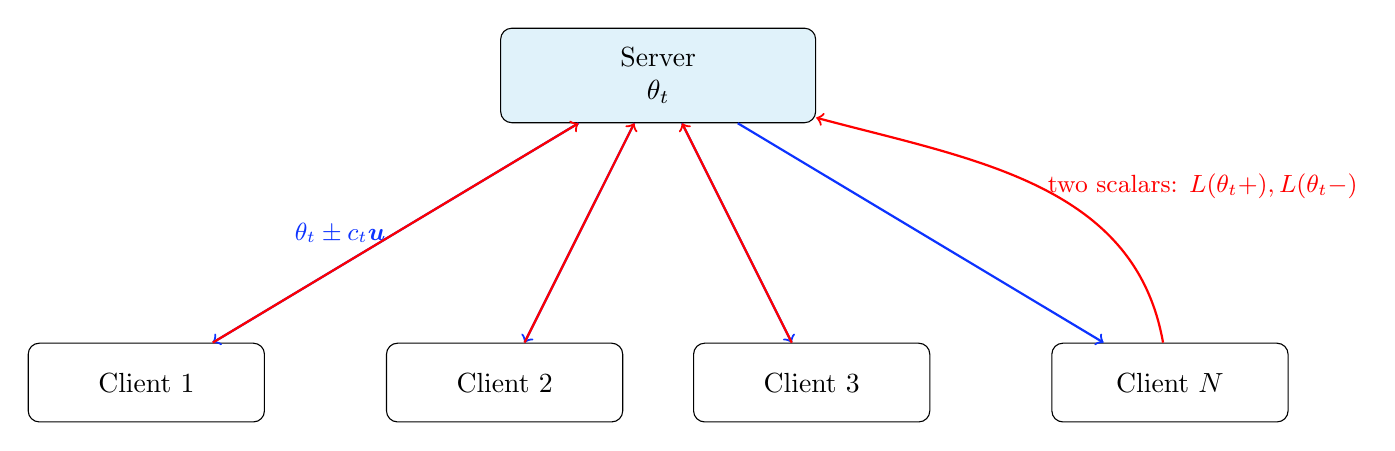
\begin{tikzpicture}[scale=1.3, every node/.style={font=\normalsize}]
	  \node[draw,rounded corners,fill=skyblue,minimum width=4cm,minimum height=1.2cm,align=center] (server) at (0,3) {Server\\$\theta_t$};
	  \node[draw,rounded corners,fill=white,minimum width=3cm,minimum height=1cm,align=center] (c1) at (-5,0) {Client 1};
	  \node[draw,rounded corners,fill=white,minimum width=3cm,minimum height=1cm,align=center] (c2) at (-1.5,0) {Client 2};
	  \node[draw,rounded corners,fill=white,minimum width=3cm,minimum height=1cm,align=center] (c3) at (1.5,0) {Client 3};
	  \node[draw,rounded corners,fill=white,minimum width=3cm,minimum height=1cm,align=center] (c4) at (5,0) {Client $N$};
	  \draw[->,thick,blue] (server) -- (c1) node[midway,left,font=\small] {$\theta_t \pm c_t\bm{u}$};
	  \draw[->,thick,blue] (server) -- (c2);
	  \draw[->,thick,blue] (server) -- (c3);
	  \draw[->,thick,blue] (server) -- (c4);
	  \draw[->,thick,red] (c1) -- (server);
	  \draw[->,thick,red] (c2) -- (server);
	  \draw[->,thick,red] (c3) -- (server);
	  \draw[->,thick,red] (c4) to[out=100,in=-15] node[midway,right,font=\small] {two scalars: $L(\theta_t{+}), L(\theta_t{-})$} (server);
	\end{tikzpicture}
	\end{center}
	\centerline{\footnotesize Figure 1: each round, clients return two loss scalars, never a gradient.}
}

\headerbox{Results}{name=results,column=1,span=2,below=methodology, above=bottom}{
	\begin{center}
	\small
	\begin{tabular}{lcccc}
	\toprule
	Method & CIFAR-100 & 20 Newsgroups & Reconstruction MSE $\uparrow$ & MI attack AUC $\downarrow$ \\
	\midrule
	FedAvg (gradient sharing) & 71.4\% & 68.9\% & 0.004 & 0.91 \\
	FedAvg + DP-SGD ($\epsilon{=}4$) & 65.2\% & 63.1\% & 0.31 & 0.58 \\
	\textbf{\textsc{ShareLess} (ours)} & \textbf{69.6\%} & \textbf{67.3\%} & \textbf{0.58} & \textbf{0.55} \\
	\bottomrule
	\end{tabular}
	\end{center}
	\centerline{\footnotesize Table 1: accuracy vs.\ two privacy metrics, averaged over 5 seeds.}

	\begin{llist}
		\item Within 1.8 points of gradient-sharing FedAvg on both tasks
		\item Membership-inference attack AUC drops from 0.91 to 0.55,
		  close to the 0.50 random-guess baseline
		\item No differential-privacy noise added — the protocol itself is
		  the mitigation, not a post-hoc perturbation
	\end{llist}
}

\headerbox{Conclusion}{name=conclusion,column=3}{
	Restricting client responses to scalar loss values, rather than
	gradients, closes most of the gap between FedAvg's accuracy and
	DP-SGD's privacy — without an explicit privacy budget to tune. The
	main cost is more communication rounds, since zeroth-order estimates
	are noisier per step than true gradients.
}

\headerbox{Demonstration}{name=demonstration,column=3,below=conclusion, above=bottom}{
	\begin{center}
		\footnotesize Code and configs: \url{https://github.com/example/shareless}
	\end{center}
}

\end{poster}

\end{document}
